%++++++++++++++++++++++++++++++++++++++++
% Don't modify this section unless you know what you're doing!
\documentclass[letterpaper,12pt]{article}
\usepackage{tabularx} % extra features for tabular environment
\usepackage{amsmath}  % improve math presentation
\usepackage{graphicx} % takes care of graphic including machinery
\usepackage[margin=1in,letterpaper]{geometry} % decreases margins
\usepackage{cite} % takes care of citations
\usepackage[final]{hyperref} % adds hyper links inside the generated pdf file
\usepackage[numbib,nottoc]{tocbibind}
\usepackage{longtable}
\usepackage{float}
\usepackage{listings}
\hypersetup{
	colorlinks=true,       % false: boxed links; true: colored links
	linkcolor=blue,        % color of internal links
	citecolor=blue,        % color of links to bibliography
	filecolor=magenta,     % color of file links
	urlcolor=blue         
}
%++++++++++++++++++++++++++++++++++++++++


\begin{document}

\title{ADMT 2018 - Project report}
\author{Group 02: Andreas Vieider (13177) \& Laurin Stricker (13412)}
\date{\today}
\maketitle

% \begin{abstract}

% \end{abstract}


\section{Introduction}

The domain of our fictional company is the one of furniture production and retail. The company is located in the province of Bolzano and has several showrooms in the area and one production center.

\subsection{Business processes}

\subsubsection{CRM - Showroom visit}

One CRM process is the collection of data about visitors at the different showrooms. A visitor can either be one who is just looking around without intention of buying anything (Seeleute), a future potential customer or an already existing customer. A visit can lead to an order.

Business questions:
\begin{itemize}
        \item Which is the best running showroom (most visitors, most orders, etc.)
        \item Where are the customers from (with different granularity)
        \item Which department are the customers the most interested in
        \item Compare the number of visitors to the number of customers for a time period and/or showroom
\end{itemize}

\subsubsection{Production}

The company logs every step in the production process, especially duration, defects and machine failures.

Business questions:
\begin{itemize}
        \item What is the average time to produce a particular product
        \item Which is the product with the highest/lowest quality
        \item How much effort/time is spent per order
\end{itemize}

\section{Conceptual Design}

\begin{longtable}{p{3cm}p{6cm}p{4cm}}
        \caption{Fact table}
        \label{tab:tabFactTable} \\
        \hline
        \toprule
        Fact & Dimensions & Measures \\
        \midrule
        \endfirsthead
        \toprule
        Fact & Dimensions & Measures \\
        \midrule
        \longtableheader
        \addlinespace
        \endhead
        \hline
        Showroom visit & Date, Showroom, Visitor, Order, Detail, Department, Sales representative & Duration (AVG), Amount of people (SUM, AVG) \\
        \hline
        Production & Start Date, End date, Product, Production Stage, Machine, Quality control, Operator & Duration (AVG), Raw material cost (AVG) \\
        \hline
\end{longtable}

\begin{figure}[H] 
        \centering
        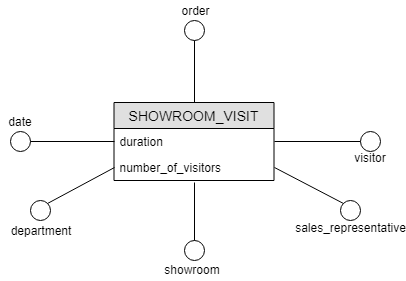
\includegraphics[scale=0.65]{../images/DFM_Showroom_Simple.png}
        \caption{
                \label{fig:showroom}  
                DFM of the showroom visit
        }
\end{figure}

\begin{figure}[H] 
        \centering
        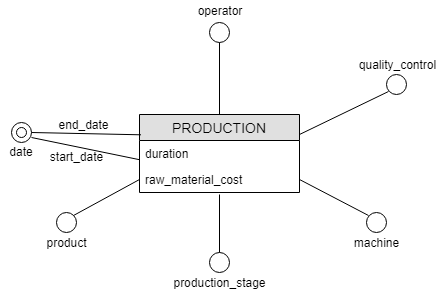
\includegraphics[scale=0.65]{../images/DFM_Production_Simple.png}
        \caption{
                \label{fig:production}  
                DFM of the production
        }
\end{figure}

\subsection{Showroom visit}

\begin{longtable}{p{4cm}p{9cm}}
        \caption{Fact table}
        \label{tab:tabShowroom} \\
        \hline
        \toprule
        Dimension & Attributes \\
        \midrule
        \endfirsthead
        \toprule
        Dimension & Attributes \\
        \midrule
        \longtableheader
        \addlinespace
        \endhead
        \hline
        Date & Day, Month, Year, Quartal, Week, Day of Week, Season, Holiday \\
        \hline
        Showroom & Name, City, District, Province, Region, Country, Manager, Address, Telephone, Size \\
        \hline
        Visitor & Name, City, District, Province, Region, Country, Language, Telephone, E-Mail, Type, Sector, Gender, Customer number \\
        \hline
        Order & Order Number, Total Price, Discount \\
        \hline
        Order Detail & Quantity, Quantity Type, Product, Unit price, Total price \\
        \line
        Department & Name \\
        \hline
        Sales representative & Name, City, District, Province, Region, Country, Language, Telephone, E-Mail, Gender
        \hline
\end{longtable}

\begin{figure}[H] 
        \centering
        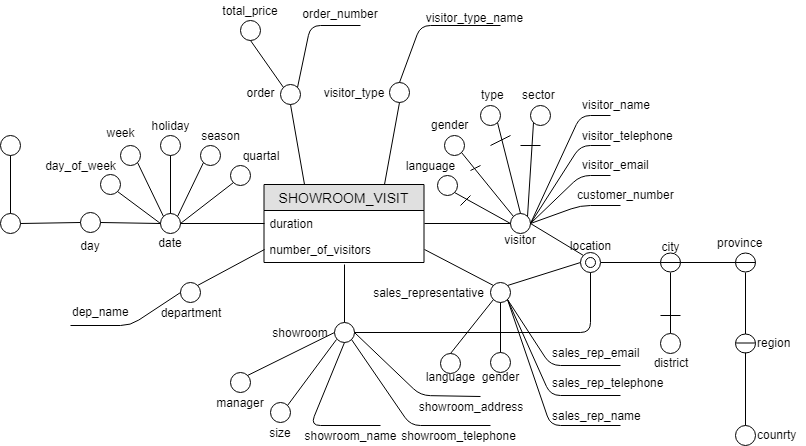
\includegraphics[width=\columnwidth]{../images/DFM_Showroom.png}
        \caption{
                \label{fig:showroomAttributes}  
                DFM of the showroom visit with attributes 
        }
\end{figure}

\subsection{Production}

\begin{longtable}{p{4cm}p{9cm}}
        \caption{Fact table}
        \label{tab:tabProduction} \\
        \hline
        \toprule
        Dimension & Attributes \\
        \midrule
        \endfirsthead
        \toprule
        Dimension & Attributes \\
        \midrule
        \longtableheader
        \addlinespace
        \endhead
        \hline
        Start date & Day, Month, Year, Week \\
        \hline
        End date & Day, Month, Year, Week \\
        \hline
        Product & Product number, Name, Department, Category \\
        \hline
        Production stage & Name \\
        \hline
        Machine & Name, Purchasing year, Vendor \\
        \line
        Quality control & Grade \\
        \hline
        Operator & Name \\
        \hline
\end{longtable}

\begin{figure}[H] 
        \centering
        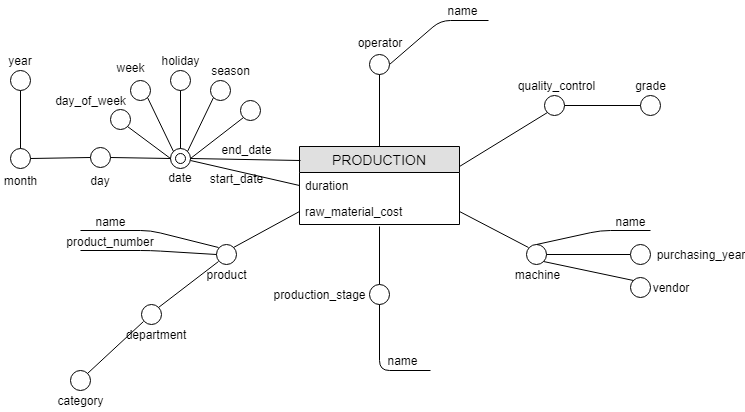
\includegraphics[width=\columnwidth]{../images/DFM_Production.png}
        \caption{
                \label{fig:productionAttributes}  
                DFM of the production with attributes 
        }
\end{figure}

\section{Logical Design}

\subsection{Star schemas}

\begin{figure}[H] 
        \centering
        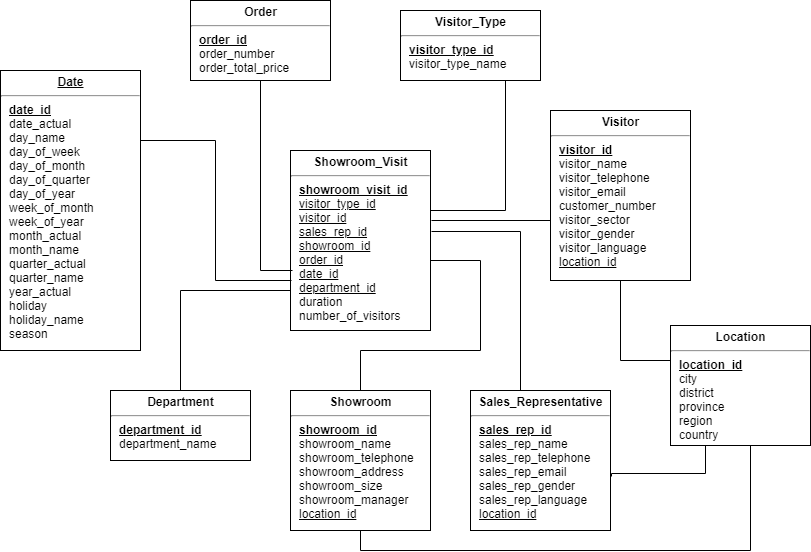
\includegraphics[width=\columnwidth]{../images/Starschema_Showroom_visit.png}
        \caption{
                \label{fig:starschemaShowroom}  
                Star schema of the showroom visit
        }
\end{figure}

\begin{figure}[H] 
        \centering
        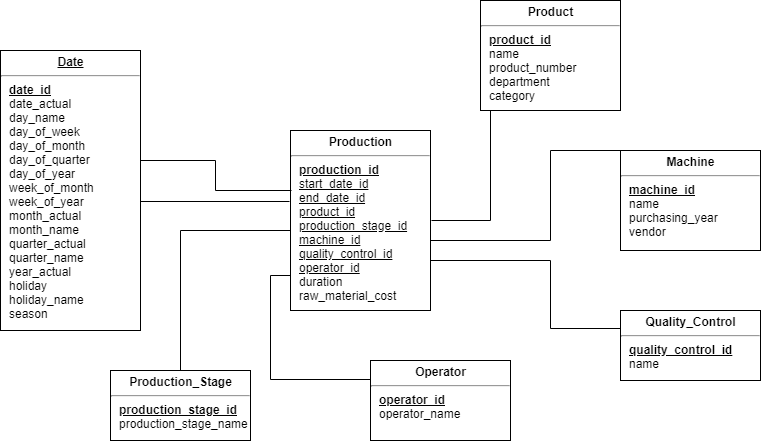
\includegraphics[width=\columnwidth]{../images/Starschema_Production.png}
        \caption{
                \label{fig:starschemaProduction}  
                Star schema of the production
        }
\end{figure}

\subsection{Two business questions}

\subsubsection{Fact: Showroom visit}

In order to be able to make the right marketing decisions, it is very important for the management to know from which sector the various customers or interested parties of a particular showroom come from. So, for example the management wants to know, from which sectors the various customers of showroom "Showroom-Bozen" were coming in the last year.

\bigskip
\noindent SQL query:
\begin{lstlisting}[
        language=SQL,
        showspaces=false,
        basicstyle=\ttfamily,
        numbers=left,
        numberstyle=\tiny,
        commentstyle=\color{gray}
     ]
        SELECT v.visitor_sector, count(*)
        FROM warehouse.visitor v
        INNER JOIN warehouse.showroom_visit sv on v.visitor_id = sv.visitor_id
        INNER JOIN warehouse.showroom s on sv.showroom_id = s.showroom_id
        INNER JOIN warehouse.date d on sv.date_id = d.date_id
        WHERE s.showroom_name = 'Showroom-BOZEN' 
        AND d.date_actual >= '2018-01-01' AND d.date_actual <= '2018-12-31'
        GROUP by v.visitor_sector
\end{lstlisting}

\begin{longtable}{p{1.4cm}p{1.5cm}p{1.8cm}p{1.5cm}p{1.6cm}p{1.4cm}p{1.2cm}p{1.25cm}p{1.85cm}}
        \caption{Showroom visit}
        \hline
        \toprule
        ID & Visitor\_id & Sales\_rep\_id & Showr.\_id & Depart.\_id & Date\_id & Type\_id & Duration & Nr.\_of\_visit. \\
        \midrule
        \endfirsthead
        \toprule
        ID & Visitor\_id & Sales\_rep\_id & Showr.\_id & Depart.\_id & Date\_id & Type\_id & Duration & Nr.\_of\_visit. \\
        \midrule
        \longtableheader
        \addlinespace
        \endhead
        \hline
        1282369	& \color{red} 570822 & 6 & \color{red} 5 & 4 & \color{red}20180323 & 2 & 90 & 2 \\
        \hline
        1282370	& 570823 & 5 & 5 & 2 & 20160107 & 4 & 167 & 4 \\
        \hline
        1282371	& 570823 & 7 & 5 & 1 & 20130526 & 3 & 173 & 6 \\
        \hline
        1282372	& 570823 & 11 & 5 & 6 & 20150806  & 3 & 100 & 10 \\
        \hline
        1282373	& 570823 & 7 & 5 & 1 & 20121116 & 4 & 169 & 5 \\
        \hline
        1282374	& 570824 & 7 & 5 & 1 & 20171210 & 3 & 57 & 3 \\
        \hline
        1282375	& 570824 & 18 & 5 & 2 & 20110212 & 3 & 166 & 7 \\
        \hline
        1282376	& 570824 & 9 & 5 & 4 & 20130811  & 3 & 84 & 5 \\
        \hline
        1282377	& 570825 & 11 & 5 & 6 & 20170507 & 3 & 184 & 10 \\
        \hline
        1282378	& 570825 & 12 & 5 & 2 & 20111127 & 2 & 26 & 2 \\
        \hline
        1282379	& 570825 & 7 & 5 & 1 & 20150425 & 3 & 141 & 10 \\
        \hline
        1282380	& 570826 & 11 & 5 & 6 & 20130208 & 2 & 8 & 2 \\
        \hline
        1282381	& 570826 & 12 & 5 & 1 & 20111214 & 3 & 61 & 8 \\
        \hline
        1282382	& 570827 & 12 & 5 & 1 & 20170202 & 3 & 139 & 9 \\
        \hline
        1282383 & 570827 & 12 & 5 & 2 & 20121012 & 3 & 71 & 7 \\
        \hline
\end{longtable}

\begin{longtable}{p{1.3cm}p{1.6cm}p{1.8cm}p{3.6cm}p{2cm}p{.7cm}p{1.2cm}p{1.5cm}}
        \caption{Visitor}
        \hline
        \toprule
        ID & Name & Telephone & E-Mail & Sector & Sex & Lang. & Loc.\_id \\
        \midrule
        \endfirsthead
        \toprule
        ID & Name & Telephone & E-Mail & Sector & Sex & Lang. & Loc.\_id \\
        \midrule
        \longtableheader
        \addlinespace
        \endhead
        \hline
        \color{red} 570822 & Melanie Eder &  &  & \color{red} Gastronomy & F & german & 9 \\
        \hline
        570823 & Julian Schmidt &  & j.schmidt@email.com & \color{red} Private & M & german & 9 \\
        \hline
        570824 & Marcel Schwarz & 306 9579783 & m.schwarz@email.com & \color{red} Hotel & M & german & 9 \\
        \hline
        570825 & Denise Fuchs & 396 5305260 & d.fuchs@email.com & \color{red} Public & F & german & 9 \\
        \hline
        570826 & Sophie Wimmer & 322 7641804 & s.wimmer@email.com & \color{red} Private & F & german & 9 \\
        \hline
\end{longtable} 

\begin{longtable}{p{0.25cm}p{3.9cm}p{2.2cm}p{2.9cm}p{.7cm}p{3.1cm}p{1.1cm}}
        \caption{Showroom}
        \hline
        \toprule
        ID & Name & Telephone & Address & Size & Manager & Loc.\_id \\
        \midrule
        \endfirsthead
        \toprule
        ID & Name & Telephone & Address & Size & Manager & Loc.\_id \\
        \midrule
        \longtableheader
        \addlinespace
        \endhead
        \hline
        1 & Showroom-LATSCH & 0477 069655 & Herrengasse 8 & 581 & Paul Wolf & 42 \\
        \hline
        2 & Showroom-M{\"U}HLBACH & 0474 039227 & Platzerstr. 58 & 349 & Christoph Steiner & 54 \\
        \hline
        3 & Showroom-M{\"O}LTEN & 0470 429676 & Vernag 97 & 857 & Christoph Steiner & 51 \\
        \hline
        4 & Showroom-SALURN & 0475 248487 & Gewerbezone 44 & 198 & Johannes Egger & 77 \\
        \hline
        \color{red} 5 & \color{red} Showroom-BOZEN & 0473 723301 & St. Urban 73 & 447 & Sabine Schneider & 9 \\
        \hline
\end{longtable} 

\begin{longtable}{p{1.6cm}p{2.1cm}p{1.4cm}p{1.5cm}p{1.6cm}p{1cm}p{1cm}p{1.1cm}p{1.2cm}}
        \caption{Date}
        \hline
        \toprule
        ID & Date & Day\_week & Day & Month & Quartal & Year & Holiday & Season \\
        \midrule
        \endfirsthead
        \toprule
        ID & Date & Day\_week & Day & Month & Quartal & Year & Holiday & Season \\
        \midrule
        \longtableheader
        \addlinespace
        \endhead
        \hline
        20160102 & 2010-01-02 & 6 & Saturday & January & First & 2016 & false & Winter \\
        20170103 & 2010-01-03 & 7 & Sunday & January & First & 2017 & false & Winter \\
        20180108 & \color{red} 2018-01-08 & 5 & Friday & January & First & 2018 & false & Winter \\
        20190109 & 2010-01-09 & 6 & Saturday & January & First & 2019 & false & Winter \\
        20200110 & 2010-01-10 & 7 & Sunday & January & First & 2020 & false & Winter \\
\hline
\end{longtable} 

\begin{longtable}{p{3cm}p{4cm}}
        \caption{Result of the query}
        \hline
        \toprule
        Sector & Number of visitors \\
        \midrule
        \endfirsthead
        \toprule
        Sector & Number of visitors \\
        \midrule
        \longtableheader
        \addlinespace
        \endhead
        \hline
        Gastronomy & 2985 \\
        Hotel & 4223 \\
        Private & 5629 \\
        Public & 1371 \\
\hline
\end{longtable} 

\subsubsection{Fact: Production}

The company's quality control is always interested in optimizing processes. It is therefore interesting for employees to know whether a machine has significant time differences in production in relation to a particular product in comparison to the other machines.

\bigskip
\noindent SQL query:
\begin{lstlisting}[
        language=SQL,
        showspaces=false,
        basicstyle=\ttfamily,
        numbers=left,
        numberstyle=\tiny,
        commentstyle=\color{gray}
     ]
     SELECT m.machine_name, avg(p.duration) as avg_production_duration
     FROM warehouse.machine m
     INNER JOIN warehouse.production p on m.machine_id = p.machine_id
     INNER JOIN warehouse.product o on p.product_id = o.product_id
     WHERE o.product_name = 'Table X'
     GROUP BY m.machine_id
\end{lstlisting}

\end{document}
